
%packages and formatting
\documentclass{article}
\usepackage{amsmath}
\usepackage{dcolumn}
\usepackage{threeparttable}
\usepackage{geometry}
\usepackage{graphicx}
\graphicspath{{../../Figures/}} % Specify the relatlive path to the "images" folder
\newcolumntype{d}[1]{D{.}{.}{#1}}
\usepackage{blindtext} % Placeholder paragraphs with text
\setlength\parindent{0pt} % No indent for new paragraphs
\usepackage{graphicx}  % for including images
\usepackage{titling}   % for more control over the title
\usepackage{float} % for tables
\usepackage{booktabs} 
\usepackage{url}

% bibliography
\usepackage[
    backend=biber,
    style=numeric,
    url=false,
    doi=false,
    eprint=false
]{biblatex}


\author{Your Name}
\date{\today}
\geometry{top=2.5cm, bottom=2.5cm}
\begin{document}

\title{\textbf{Gender Pay Gap in Switzerland}}


\begin{titlepage}
\centering

\begin{figure}[H]
    \centering
    
\includegraphics[width=0.7\textwidth]{Figures/uzhseal.png} 
    \label{fig:example}
\end{figure}
    
    \vspace{1cm}
    \Huge
    \textbf{Gender Pay Gap in Switzerland}
    
    \vspace{1cm}
    \LARGE
    This research project analyses the gender pay gap in Switzerland across industries and regions in Switzerland from 2012 to 2022. 
    
    \vspace{1cm}
    \textbf{Authors:}\\ Tanja Bekic \\  Sakshi Sachin Chaudhari
    \vspace{1cm}
    
    \textbf{Date:}\\
    \thedate
    \vfill
    
\end{titlepage}



\section{Introduction}
The gender pay gap remains a significant and persistent issue in contemporary labor markets, representing disparities in earnings between men and women. Although progress toward gender equality has been made over the years, the wage gap between men and women in Switzerland remains evident. These disparities are not only reflective of broader systemic inequalities but also have implications for social equity and economic efficiency. Understanding the scale of the gender pay gap is critical for policymakers, employers and employees. \\
This paper focuses on quantifying the gender pay gap across gross regions in Switzerland and across industries. By providing a comparative analysis of these disparities, this research seeks to identify patterns and trends that reveal where wage gaps are most pronounced. By examining these variations, the study aims to offer a clearer picture of where wage disparities are most pronounced and how they differ based on geographic and sectoral factors.  \\
Rather than investigating the underlying causes of the gender pay gap, this research paper aims to present a data-driven overview of its size and distribution. By doing so, it contributes to a foundational understanding of wage inequality in Switzerland and provides valuable insights that can inform future research and policy development.


\section{Data}

For this analysis, we require official data from the Federal Statistical Office of Switzerland. The data comes in two distinct sets, one containing data sets on gross regions in Switzerland and the other on overall Switzerland.

    \begin{itemize}
        \item  Gross monthly wage (central value) by economic division, occupational status and gender \textit{(Monatlicher Bruttolohn (Zentralwert) nach Wirtschaftsabteilungen, beruflicher Stellung und Geschlecht)}\cite{1}
        \item  Gross monthly wage (central value) by degree of employment, occupational status and gender - private and public sector combined \textit{Monatlicher Bruttolohn (Zentralwert) nach Beschäftigungsgrad, beruflicher Stellung und Geschlecht – Privater und öffentlicher Sektor zusammen} \cite{2}
        \item Gross monthly wage (central value) by degree of employment, occupational status and gender - private and public sector combined \textit{Monatlicher Bruttolohn (Zentralwert) nach Beschäftigungsgrad, beruflicher Stellung und Geschlecht - Privater und öffentlicher Sektor zusammen}\cite{3}
    \end{itemize}


The data sets on regions are provided for the following gross regions:
     \begin{itemize}
        \item Lake Geneva \textit{(Genfersee)}
        \item Midlands\textit{(Mittelland)}
        \item North West\textit{(Nordwestschweiz)}
        \item East \textit{(Ostschweiz)}
        \item Ticino \textit{(Tessin)}
        \item Central \textit{(Zentralschweiz)}
        \item Zurich \textit{(Zürich)}
    \end{itemize}
\\

The gross regions are defined by the Federal Statistical Office.\cite{1} \\
The Lake Geneva region comprises the cantons of Vaud, Valais and Geneva. Midlands comprises the cantons of Bern, Fribourg, Solothurn, Neuchatel and Jura. The cantons of Baselland, Baselstadt and Aargau are in the greater region of Northwestern Switzerland and Eastern Switzerland comprises the cantons of Glarus, Schaffhausen, Appenzell Innerrhoden and Appenzell Ausserrhoden, St. Gallen, Graubünden and Thurgau. Central Switzerland comprises the cantons of Lucerne, Uri, Schwyz, Obwalden and Nidwalden and Zug. The cantons of Zurich and Ticino are each large regions in their own right. The data sets on gross regions had to be merged into one data set.

\section{Methodology}

To analyze the gender pay gap in Switzerland, we applied data visualization techniques. These included bar and line charts, box plots and heat maps, which provided an overview of the distribution and trends in wages across genders. Through these visualizations, we identified key patterns, such as variations in pay across industries, age groups, and education levels. The visualizations served as a critical foundation for understanding the data.\\

The given data sets had missing values, these were handled in different ways: 
\begin{itemize}
        \item Missing data in the data set on gross monthly wages overall Switzerland were XXXXXXX
        \item Missing data in data sets on gross regions were removed, as the merged data set provided enough data entry points. 
\end{itemize}
\\
All visualizations in this study were tested for color accessibility using a color blindness simulator to ensure that they are interpretable by individuals with color vision deficiencies. The simulator allowed us to assess how the color choices in the charts would appear to those with common conditions. Based on the results, adjustments were made to the color palette to enhance contrast and ensure clarity for all viewers, regardless of their color vision abilities.\cite{3}\\
\\
\section{Discussion of Results}

\subsection{Gender Pay Gap Across Switzerland}

\begin{table}[H]
\centering
\resizebox{\textwidth}{!}{%
\begin{tabular}{@{}c|cc|ccc@{}}
\toprule
Statistic & Gross Pay Men & Gross Pay Women & Gender Pay Gap &  Gender Pay Gap in Percent \\ \midrule
Mean     & 61,224.99   & 47,136.34  & 15,218.60  & 21,55\% \\
Std Dev  & 27,670.40   & 22,186.11  & 12,584.60  & 19,52\%\\
Min      & 13,300.40   & 6,400      & N/A        & N/A \\
25\%     & 37,500.00   & 28,200.00  & 7,500      & 14,45\%\\
50\%     & 61,300.00   & 46,600     & 13,800     & 21,15\%\\
75\%     & 74,150.00   & 60,000     & 21,000     & 31,66\%\\
max\%    & 13,600.00   & 118,900    & 70,800.00  & 82,76\%\\
\bottomrule
\end{tabular}\\
}\
\caption{Descriptive Statistics on Gender Pay Gap Across Switzerland and Years}
\end{table}

The gender pay gap is defined as the absolute difference between the wage of men and women, while the gender pay gap in percent is defined as the relative difference between the wages of men and women.\\
\\
  1. Equation 1: \(\textit{Gender Pay Gap} = \textit{Wage Men} - \textit{Wage Women)}\)\\
  2. Equation 2: \(\textit{Gender Pay Gap in Percent} = 1 - \frac{\textit{Wage Men}} 
 {\textit{Wage Women}}\)\\
\\
The descriptive statistics of the gender pay gap in Switzerland reveal a persistent disparity in earnings between men and women across all industries and time periods examined. On average, women earn significantly less than men. \\

\begin{figure}[h]
    \centering
    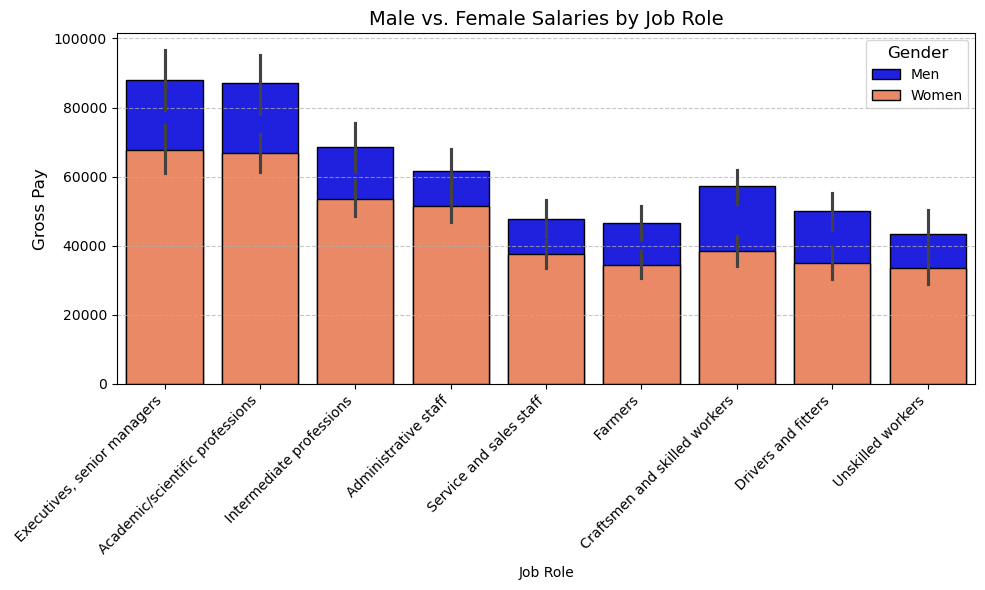
\includegraphics[width=1\textwidth]{Figures/Salaries_by_Job_Role.png}
    \caption{Gender Pay Gap by Job Role}
    \label{fig:pay_gap_roles}
\end{figure}

Significant disparities emerge across occupational categories when analyzing the gender pay gap by job roles in Switzerland. The largest gap is observed among \textit{Craftsmen and Skilled Workers}, where women earn, on average, 34.59\% less than men, highlighting a pronounced inequality in traditionally male-dominated roles. Similarly, high gaps are evident in \textit{Academic/Scientific Professions} (22.49\%) and \textit{Executives and Senior Managers} (22.37\%), suggesting that even in highly educated or leadership positions, gender-based pay inequities persist. It is important to note that these statistics do not control for differences in full-time versus part-time employment, which could partially explain the higher observed pay gaps in certain roles, particularly those where part-time work is more common among women.\\


 Figure \ref{fig:pay_gap_roles} displays the absolute wage values across job roles, providing a clear representation of the gross pay for men and women in each occupation. It allows for a direct comparison of earnings in monetary terms, highlighting the overall wage levels within each job role.\\

Figure \ref{relative_gap_roles}, on the other hand, presents the relative gender pay gap for the same job roles, illustrating the percentage difference in earnings between men and women. By focusing on the relative gap, this figure enables a deeper understanding of the proportional disparity in wages, independent of the absolute wage levels. Together, these figures offer complementary insights into both the overall pay distribution and the extent of gender-based wage inequalities across different job categories.\\

\begin{figure}[h]
    \centering
    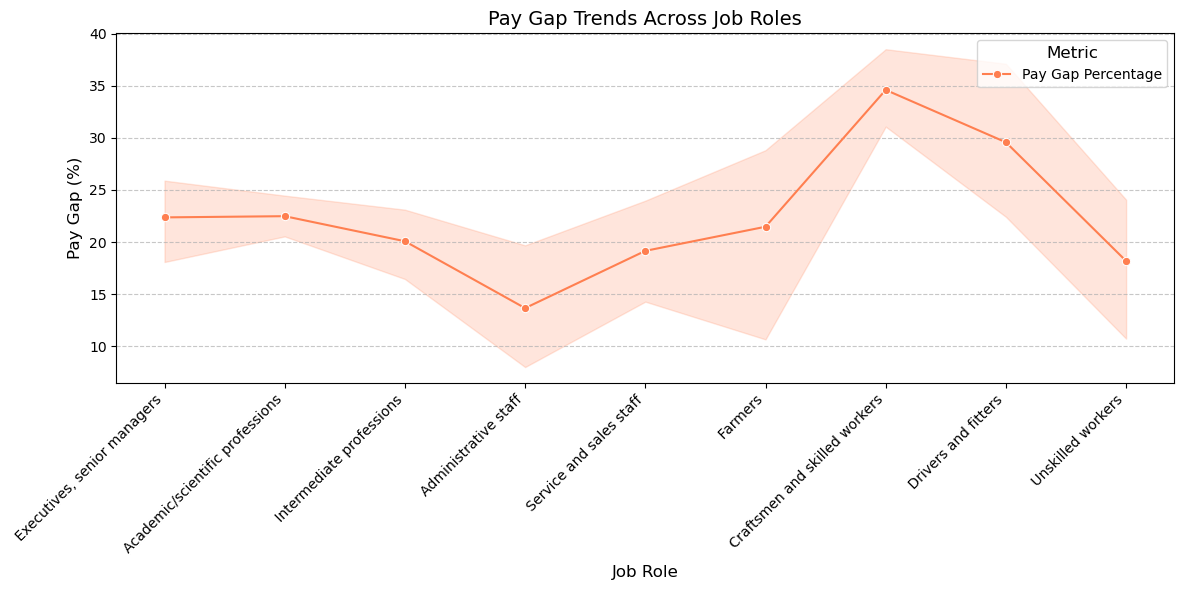
\includegraphics[width=1\textwidth]{Figures/Pay_Gap_Trends_by_Job_Role.png}
    \caption{Relative Gender Pay Gap by Job Role}
    \label{relative_gap_roles}
\end{figure}

The relative gender pay gap by job role offers a clear depiction of the percentage disparities across various occupational categories, alongside the variations within each category. Even though the gender pay gap of \textit{craftsmen and skilled workers} is the largest (34.59\%), it has the smallest variation across all categories.\\


The high relative gender pay gap among \textit{craftsmen and Skilled Workers} can be attributed to several structural and societal factors. First, this group aggregates very diverse specific job roles across various industries. These roles are often male-dominated and associated with traditional gender norms. In addition, skilled worker roles often involve pay structures influenced by seniority and overtime. The lack of control over full-time versus part-time employment in this analysis further compounds this issue, as women in these roles are more likely to work part-time, reducing their average earnings relative to men. Finally, cultural biases and systemic discrimination in traditionally male-oriented trades may also contribute to the significant disparities observed in this category.\\

The relatively smaller gender pay gap among \textit{administrative staff} can likely be attributed to several factors. First, administrative roles often have more standardized pay structures, such as set salary scales or fixed hourly wages, which leave less room for negotiation or discretionary pay that could introduce gender-based disparities. Furthermore, these roles may exhibit less occupational segregation compared to other categories, as they tend to attract a more balanced gender distribution and involve tasks that are not strongly associated with traditional gender norms. Additionally, administrative positions may have fewer hierarchical levels, reducing the opportunities for unequal advancement or promotions that contribute to larger gaps in other sectors, such as executive or academic roles. \\


\begin{figure}[h]
    \centering
    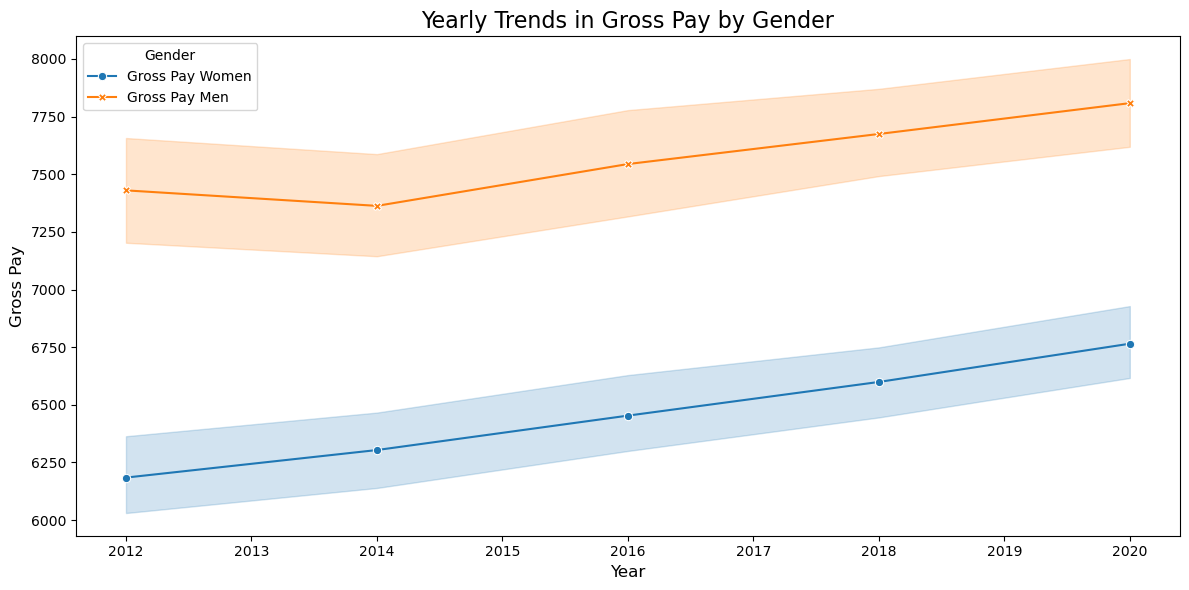
\includegraphics[width=1\textwidth]{Figures/Trends_Gross_Pay_Gender.png}
    \caption{Trends in Gross Pay by Gender over Years}
    \label{fig:gross_trend}
\end{figure}

Figure  \ref{fig:gross_trend} visualizes the trend of gross pay across all industries in Switzerland over time. It reveals an upward trend in wages for both men and women. However, the persistent gap between the two lines underscores the enduring gender pay gap, with men consistently earning higher wages than women. Despite this disparity, the decreasing distance between the lines over time demonstrates a gradual narrowing of the pay gap, suggesting progress toward greater gender wage equality.\\

\begin{figure}[h]
    \centering
    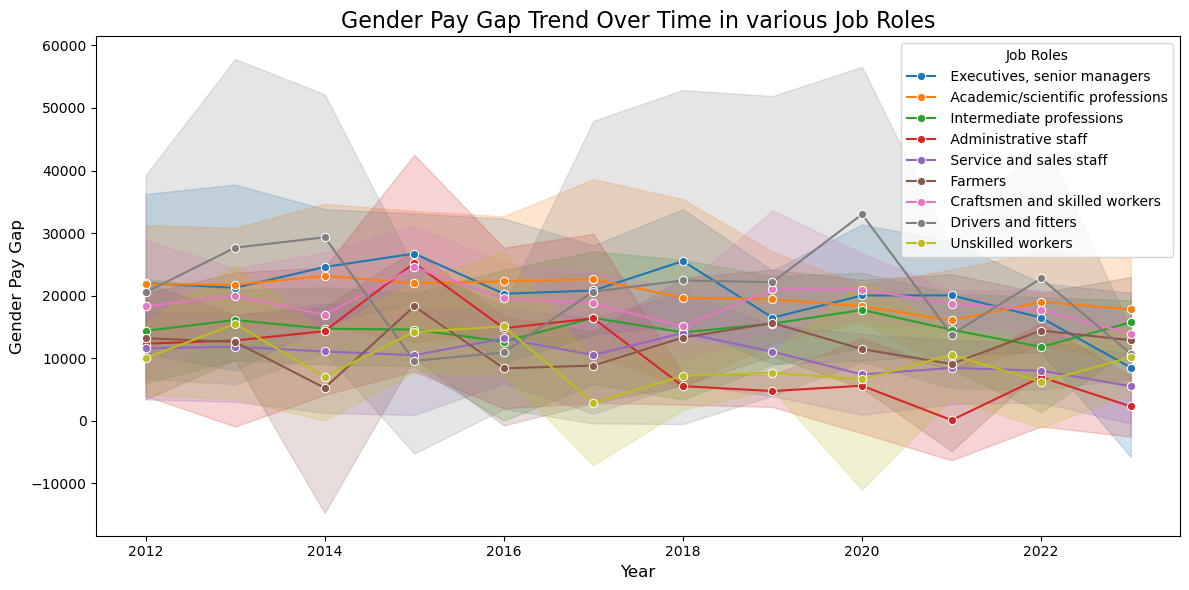
\includegraphics[width=1\textwidth]{Figures/Gap_over_Time_Roles.png}
    \caption{Trends in Gender Pay Gap by Job Roles over Years}
    \label{fig:roles_trend}
\end{figure}

 The visualization in Figure \ref{fig:roles_trend} depicting the gender pay gap over time by job role reveals that, while the absolute levels of the gender pay gap differ across occupations, the overall trend remains consistent across all job roles. Despite variations in the magnitude of the gap between job categories, there are no significant deviations in the trend lines, indicating that the narrowing of the pay gap occurs uniformly across different sectors. This suggests that, although certain roles have higher or lower initial disparities, the factors driving the reduction in the gender pay gap are broadly applicable across various occupations. None of the job roles stands out as experiencing a disproportionately large or small reduction in the gap, reinforcing the notion that progress toward wage equality is generally occurring at a similar pace across the labor market.\\


\begin{figure}[h]
    \centering
    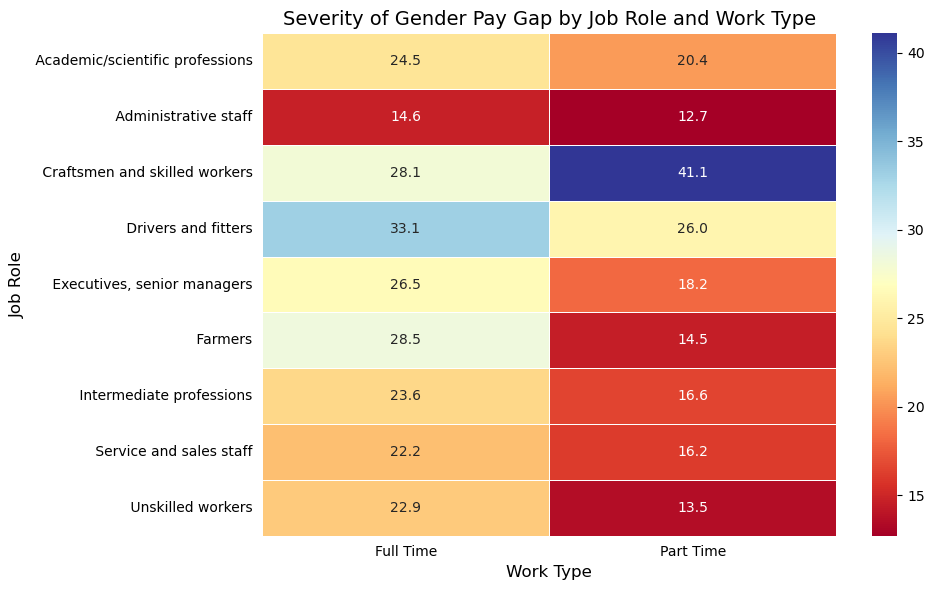
\includegraphics[width=0.8\textwidth]{Figures/Severity_of_Pay_Gap_by_Role_and_Work_Type.png}
    \caption{Relative Gender Pay Gap by Job Role and Work Tipe}
    \label{fig:heatmap}
\end{figure}

The Federal Statistical Office defines part-time work as any employment up to 80\% of a full-time workload, while full-time work is classified as 90-100\% of a standard work schedule \cite{3}. Figure \ref{fig:heatmap} segregates the data into full-time and part-time workers as well as the defined job roles.  It provides key insights into how employment type influences the gender pay gap across professions. \\
In \textit{Academic/Scientific Professions}, the relatively small pay gap difference between full-time and part-time positions suggests that wage structures in this category are less influenced by working hours or employment type. Academic roles often have standardized salary scales tied to qualifications and seniority, rather than hourly or performance-based metrics, which may mitigate disparities between full-time and part-time workers. Moreover, part-time positions in academia may still require high qualifications and specialized expertise, ensuring comparable pay rates. \\
\\
In contrast, the gender pay gap is starkly pronounced in \textit{Craftsmen and Skilled Workers}, where it reaches 28.1\% for full-time roles and escalates to 41.1\% for part-time positions. This significant difference can be attributed to structural and cultural factors within this industry. Part-time roles in skilled professions may often be lower-skilled or less senior positions, which women are more likely to occupy, resulting in wider pay disparities. Additionally, part-time workers in this field may have limited access to bonuses or specialized training opportunities, further exacerbating the gap. The male-dominated nature of these professions also likely contributes to systemic inequalities in wages, promotions, and the valuation of work performed by women, particularly in less visible or part-time roles.\\

In Figure \ref{fig:distribution_gross}, the distributions of gross wages per job role are further differentiated by gender. A wider box indicates greater variability within a job role category on a gender while the length of the whiskers, which extend from the box to the minimum and maximum values provide information about wage dispersion. Longer whiskers indicate greater variability in pay at the extremes within a group. Longer whiskers may indicate a higher impact of seniority on the wages or higher bargaining power in a job role. \\
\\
In category \textit{Executives, senior managers}, the variability between men and women is the largest. The width of the boxes indicates a wider range of salaries within male, compared to female, suggesting that men are more likely to occupy higher-paying senior positions and more variable roles within executive levels. The long whiskers, extending to both higher and lower extremes of the pay scale, further emphasize this variability on male executives.In contrast, the box for women is smaller, indicating less variability in pay among female executives and senior managers. However, the whiskers for women are longer than those for men, which suggests a broader spread of salaries at the extremes within the female group. \\
Despite the lengther wisker for women, the absolute value of the whisker remains smaller than the one for men, indicating that fewer women occupy the highest-paying positions within this category. This disparity in the upper pay distribution highlights the underrepresentation of women in the highest-paying senior roles, reinforcing the notion of a "glass ceiling" effect. 
\clearpage

\begin{figure}[t]
    \centering
    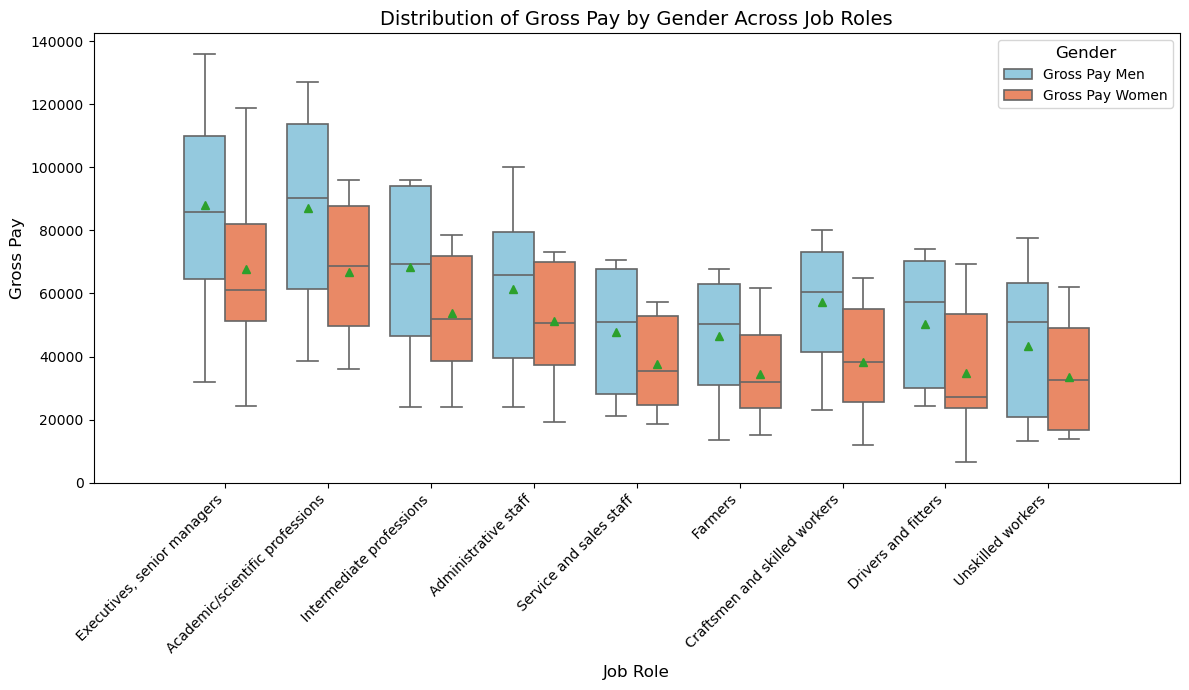
\includegraphics[width=1\textwidth]{Figures/Distribution_Gross-Pay.png}
    \caption{Distribution of Gender Pay Gap by Job Role and Work Type}
    \label{fig:distribution_gross}
\end{figure}



\subsection{Gender Pay Gap Across Gross Regions in Switzerland}

\begin{figure}[t]
    \centering
    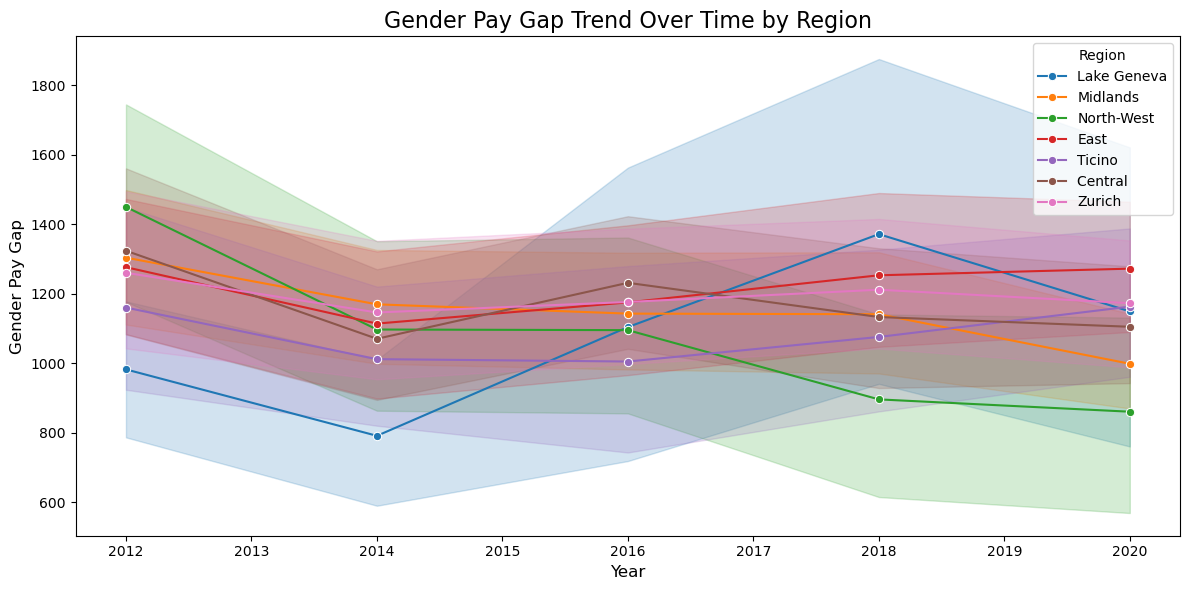
\includegraphics[width=1\textwidth]{Figures/Pay_Gap_Over_Time_Region.png}
    \caption{Gross Gender Pay Gap over Time Across Gross Regions in Switzerland}
    \label{fig:trend_regions}
\end{figure}
\\
\\
A downward trend in the gender pay gap across Switzerland's gross regions over time can be observed in Figure \ref{fig:trend_regions}. This suggests a gradual reduction in wage disparities between men and women. This overall decline could be attributed to several factors, including increasing awareness of gender equality and growing social pressures for more equitable pay practices. The trend also likely reflects broader shifts in societal attitudes towards gender roles, with more women entering higher-paying industries and occupations.\\
\\
The largest decline in the gender pay gap is found in the North-West region and may be linked to several regional factors. This area includes the city of Basel, its agglomerations and the canton of Aargau, which all are home to a high concentration of multinational corporations in the pharmaceutical, finance and technology sectors. These employers may have increasingly adopted progressive policies around gender pay equity. Furthermore, this region may have seen a greater number of women entering high-paying sectors and leadership roles, contributing to the narrowing of the pay gap.\\

Figure\ref{fig:gap_regions} depicts the absolute gender pay gap across Swiss regions and illustrates that the disparities in wages between men and women are relatively consistent nationwide, with no region displaying significantly higher or lower gaps. This suggests that the gender pay gap is a pervasive issue across Switzerland, driven by systemic factors that are not confined to specific geographic areas.\\

\begin{figure}[h]
    \centering
    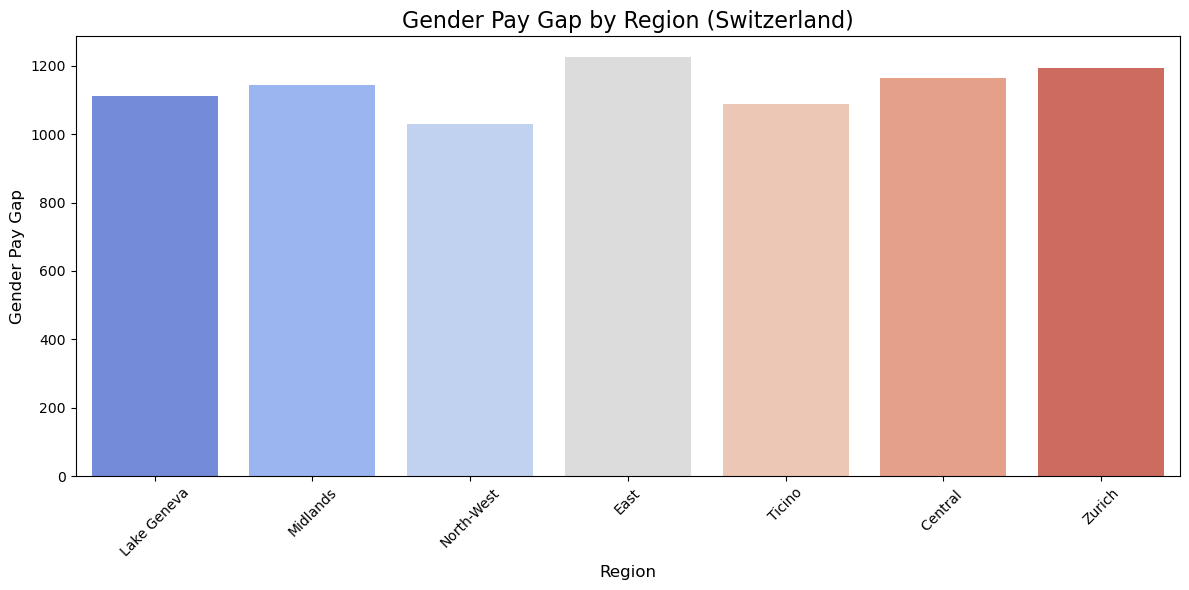
\includegraphics[width=0.7\linewidth]{Figures/Gross_Pay_Gap_Region.png}
    \caption{Gender Pay Gap by Region}
    \label{fig:gap_regions}
\end{figure}
\\
Similarly, the subsequent Figure \ref{fig:ratio_region}, which presents the gross pay ratio between men’s and women’s wages across regions, reinforces this finding. The ratio consistently falls between 0.8 and 0.9 across all regions, indicating that women earn approximately 80-90\% of what men earn. While this ratio underscores the existence of a substantial gender pay gap, the lack of significant variation between regions suggests that national-level policies and cultural norms exert a homogenizing influence on wage disparities, regardless of regional economic or industrial differences.\\
\begin{figure} 
    \centering
    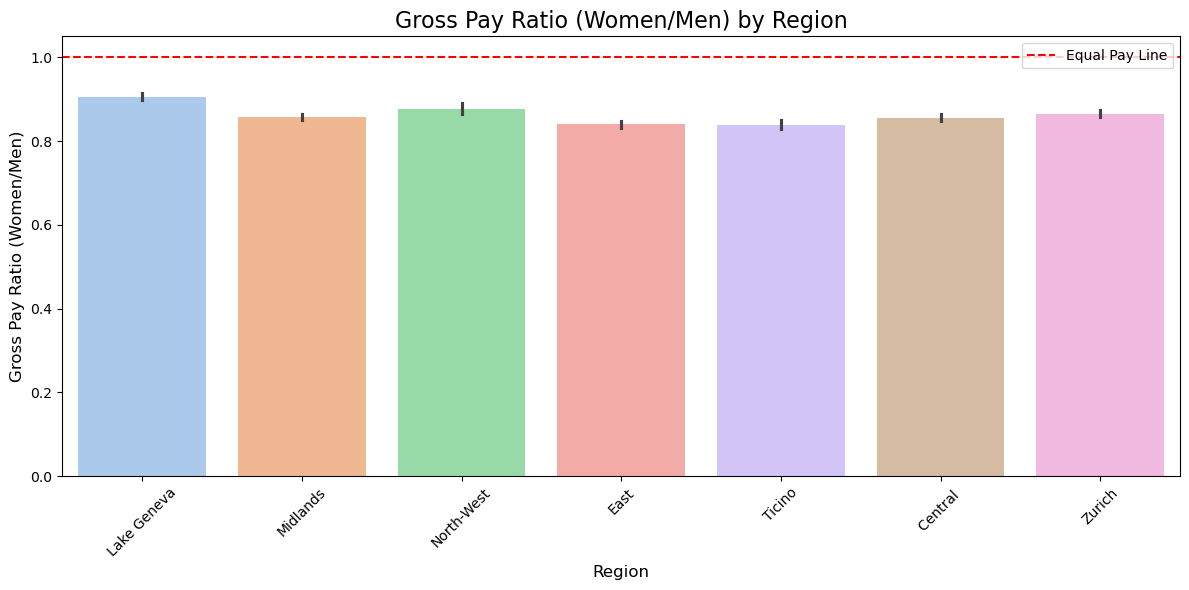
\includegraphics[width=0.7\linewidth]{Figures/Gross_Ratio_Region.png}
    \caption{Ratio of Gross Wages by Region}
    \label{fig:ratio_region}
\end{figure}
\\


\clearpage
\section{Conclusion}

This study confirms the existence of a persistent gender pay gap in Switzerland, highlighting disparities in wages between men and women across various dimensions. Significant differences are observed across industries, with certain sectors showing high variations in the gender pay gap. However, the industries with high variation summarize a diverse range of occupations. \\

Over the observed time frame, the gender pay gap has shown a gradual decrease, reflecting positive, though slow, progress toward wage equality. Regional differences in the pay gap were identified, but the variations in absolute terms were found to be relatively minor, indicating that regional disparities are less pronounced than those seen across industries. \\

It is important to note that this analysis provides an overview of the descriptive statistics, offering valuable insights into the observed patterns but without controlling for confounding variables such as working hours, education, experience or age. Future research is needed to explore these underlying factors and their contributions to the gender pay gap in greater detail.


% Bibliography section
\newpage  % Start a new page for the bibliography
\section{References}


\begin{thebibliography}{9} % Zahlen gibt den Platz für Referenzen an

\bibitem{Regions} Bundesamt für Statistik (BFS). (2023). Lohnstruktur nach Grossregionen. \\
Retrieved on 6. December 2024 from  \url{https://www.bfs.admin.ch/bfs/de/home/statistiken/arbeit-erwerb/loehne-erwerbseinkommen-arbeitskosten/lohnstruktur/grossregionen.html}

\bibitem{GrossPay} Bundesamt für Statistik (BFS). (2023). Monatlicher Bruttolohn (Zentralwert) nach Beschäftigungsgrad, beruflicher Stellung und Geschlecht – Privater und öffentlicher Sektor zusammen. \\
Retrieved on 6. December 2024 from \url{https://www.bfs.admin.ch/bfs/de/home/statistiken/kataloge-datenbanken.assetdetail.30385239.html}

\bibitem{PartTime}Bundesamt für Statistik (BFS). (2023). Monatlicher Bruttolohn (Zentralwert) nach Beschäftigungsgrad, beruflicher Stellung und Geschlecht – Privater und öffentlicher Sektor zusammen. Retrieved on 6. December 2024 from
\url{https://www.bfs.admin.ch/bfs/de/home/statistiken/kataloge-datenbanken.assetdetail.30385239.html}

\bibitem{ColorBlindness} Color Blindness. (2023). Coblis - Color Blindness Simulator. Retrieved on 6. December 2024 from \url{https://www.color-blindness.com/coblis-color-blindness-simulator/}

\end{thebibliography}



\end{document}

\end{document}